\documentclass{beamer}
%\documentclass[aspectratio=169]{beamer}
\mode<all>
{
  \usetheme{default}      % or try Darmstadt, Madrid, Warsaw, ...
  \usecolortheme{default} % or try albatross, beaver, crane, ...
  \usefonttheme{default}  % or try serif, structurebold, ...
  \setbeamertemplate{navigation symbols}{}
  \setbeamertemplate{caption}[numbered]
  \setbeamertemplate{itemize items}[circle]
  \setbeamertemplate{frametitle}{\textbf{\insertframetitle}\\\small\insertframesubtitle}
  %\setbeamertemplate{frametitle}{\bfseries\insertframetitle\par}
}

\usepackage[english]{babel}
\usepackage[utf8]{inputenc}
%\usepackage[T1]{fontenc}

\usepackage{framed}
\usepackage{amssymb}
\usepackage{amsmath}
\usepackage{amsthm}
\usepackage{graphicx}
\usepackage{makecell}
\usepackage{wrapfig}
\usepackage{float}
\usepackage{booktabs}

\newcommand\Wider[2][3em]{%
\makebox[\linewidth][c]{%
  \begin{minipage}{\dimexpr\textwidth+#1\relax}
  \raggedright#2
  \end{minipage}%
  }%
}


\title{\textbf{FunSearch \& AlphaEvolve}}
\author{
\textbf{
Bartosz Piotrowski
}}
\date{
August 21, 2025\\
The Reasoning Reading Group @ FAIR
}

\begin{document}

\begin{frame}
  \titlepage
\end{frame}

\begin{frame}{Motivation}
Preconditions:
\begin{itemize}
\item A problem of finding optimal heuristic / program / function.
\item A pre-trained, coding-capable LLM.
\item An automated evaluator returning a scalar score.
\end{itemize}
\pause
The simplest strategy:
\begin{itemize}
\item generating multiple independent samples from the LLM with non-zero
 temperature,
\item evaluating all of them,
\item selecting the best one.
\end{itemize}

\pause
But instead of sampling independently, can we \textbf{incorporate the evaluator
feedback} into subsequent generations?

\end{frame}

\begin{frame}{FunSearch}
Key ingredients:
\begin{itemize}
\item \textit{best-shot} prompting,
\item a growing database of programs,
\item an evolutionary strategy acting on it.
\end{itemize}
\end{frame}

\begin{frame}{FunSearch}
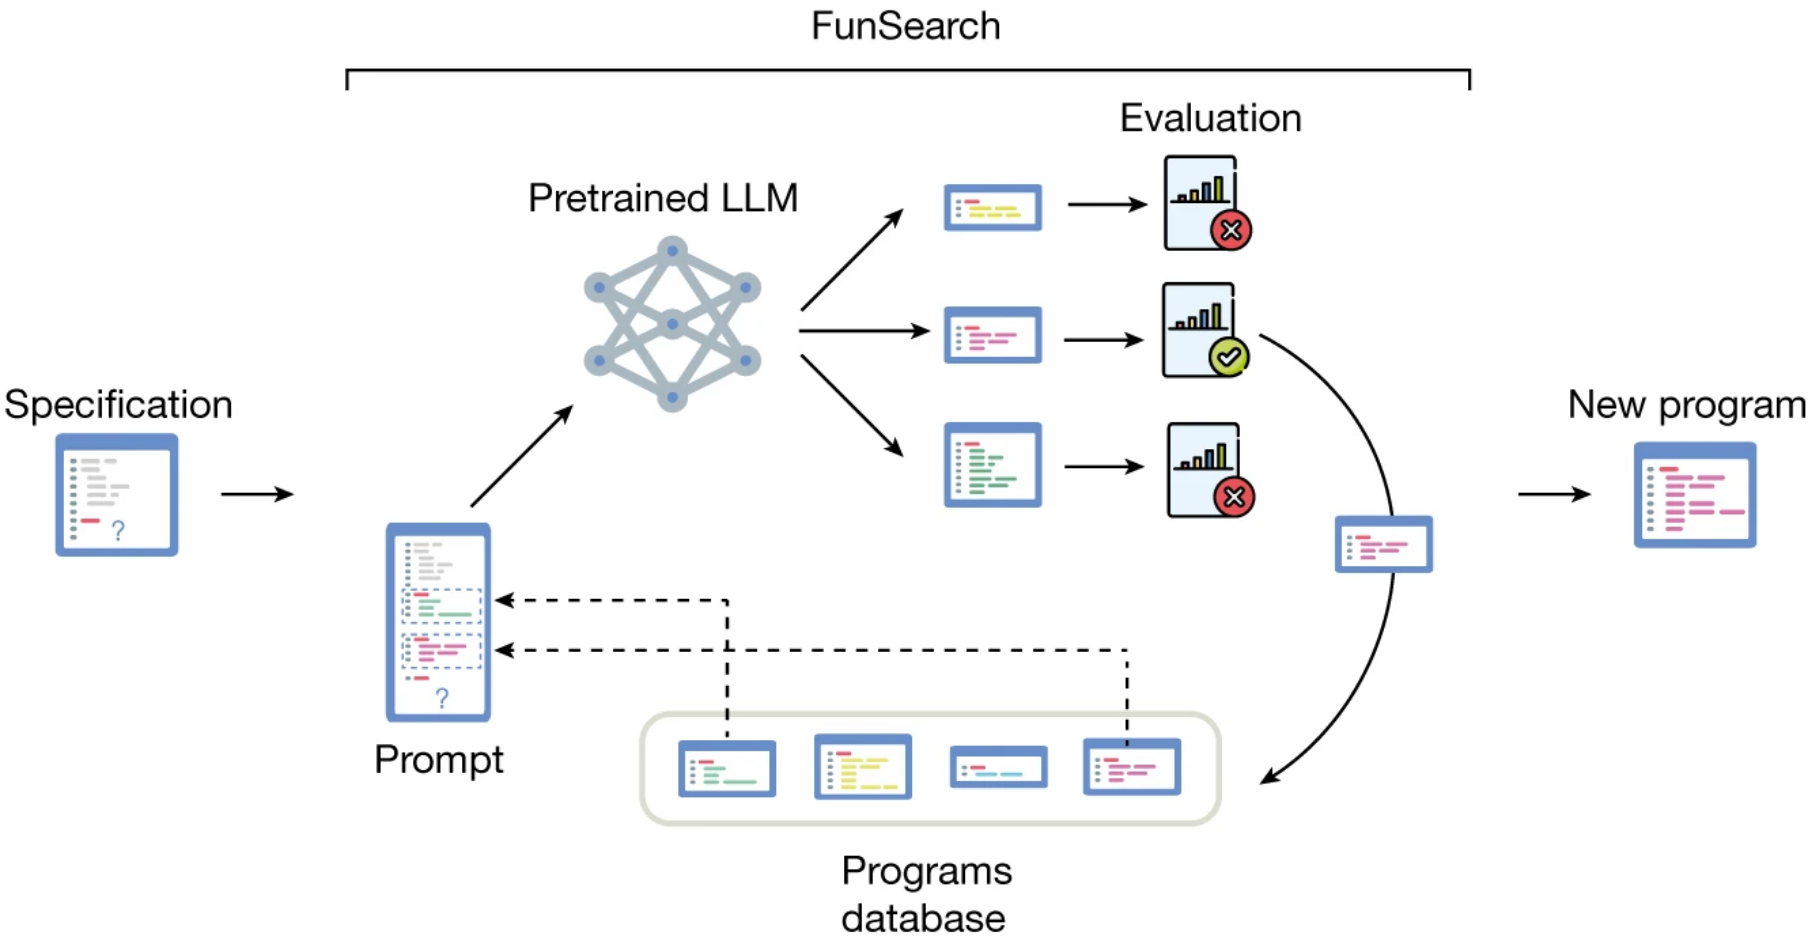
\includegraphics[width=\linewidth]{figures/funsearch-overview.png}
\end{frame}

\begin{frame}{Database of programs}
\begin{itemize}
\item Several islands/subpopulations growing independently.
\item Higher-scoring programs, but also shorter ones, are prioritized.
\item Less good programs are eventually discarded.
\item Different islands are mixed with each other to an extent.
\item Why multiple islands? For diversity.
\end{itemize}
\end{frame}

\begin{frame}{Best-shot prompting}
\begin{itemize}
\item $k$ good programs per prompt sampled, for each island.
\item Information which one is better incorporated into the prompt (\textit{v0,
v1, \ldots}).
\item In the actual experiments, $k = 2$.
\end{itemize}
\end{frame}

\begin{frame}{Other details}
\begin{itemize}
\item \textbf{Model:}
\begin{itemize}
\item Codey, a PaLM2 model fine-tuned on code.
\item Smaller, faster-inference model chosen.
\end{itemize}
\item Implementation with \textbf{three asynchronous workers:}
\begin{itemize}
\item database,
\item generator,
\item evaluator.
\end{itemize}
\item Prompting with \textbf{templates / skeletons of programs}.
\begin{itemize}
\item The LLM asked to modify only the essential function.
\end{itemize}
\end{itemize}
\end{frame}

\begin{frame}{Problems tackled}
Two known combinatorics problems:
\begin{itemize}
\item Cap set problem.
\item (Online) bin packing.
\end{itemize}
\end{frame}

\begin{frame}{Cap set problem}
What is the largest possible set of vectors in $\mathbb{Z}^n_3$
 (\textit{cap set}) such that no three vectors sum to zero?
\pause
\begin{figure}
    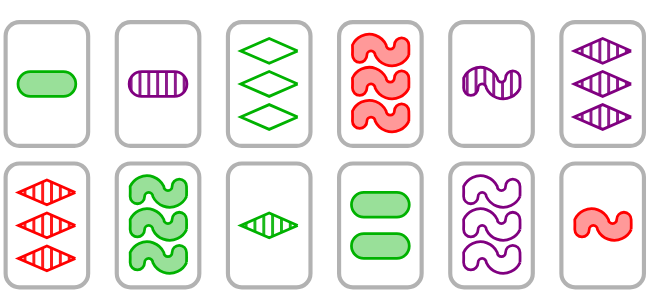
\includegraphics[width=0.6\linewidth]{figures/no-set.png}
\end{figure}
    \pause
\begin{figure}
    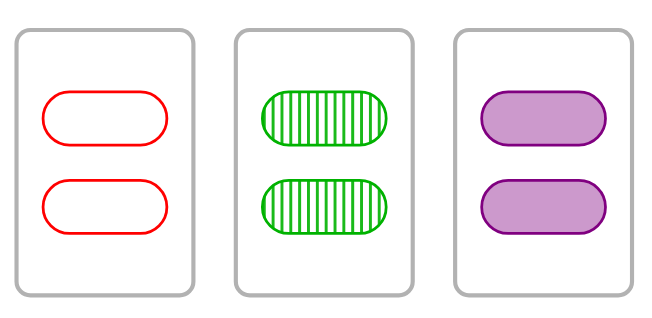
\includegraphics[width=0.4\linewidth]{figures/set.png}
\end{figure}
\pause
\begin{figure}
\centering
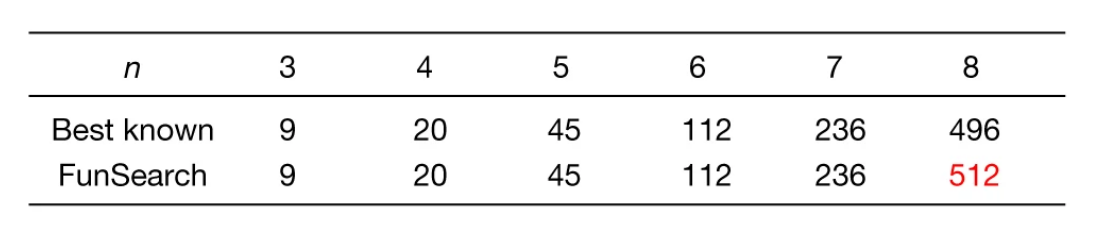
\includegraphics[width=0.7\linewidth]{figures/cup-set-table.png}
\end{figure}
\end{frame}


\begin{frame}{Cap set problem template}
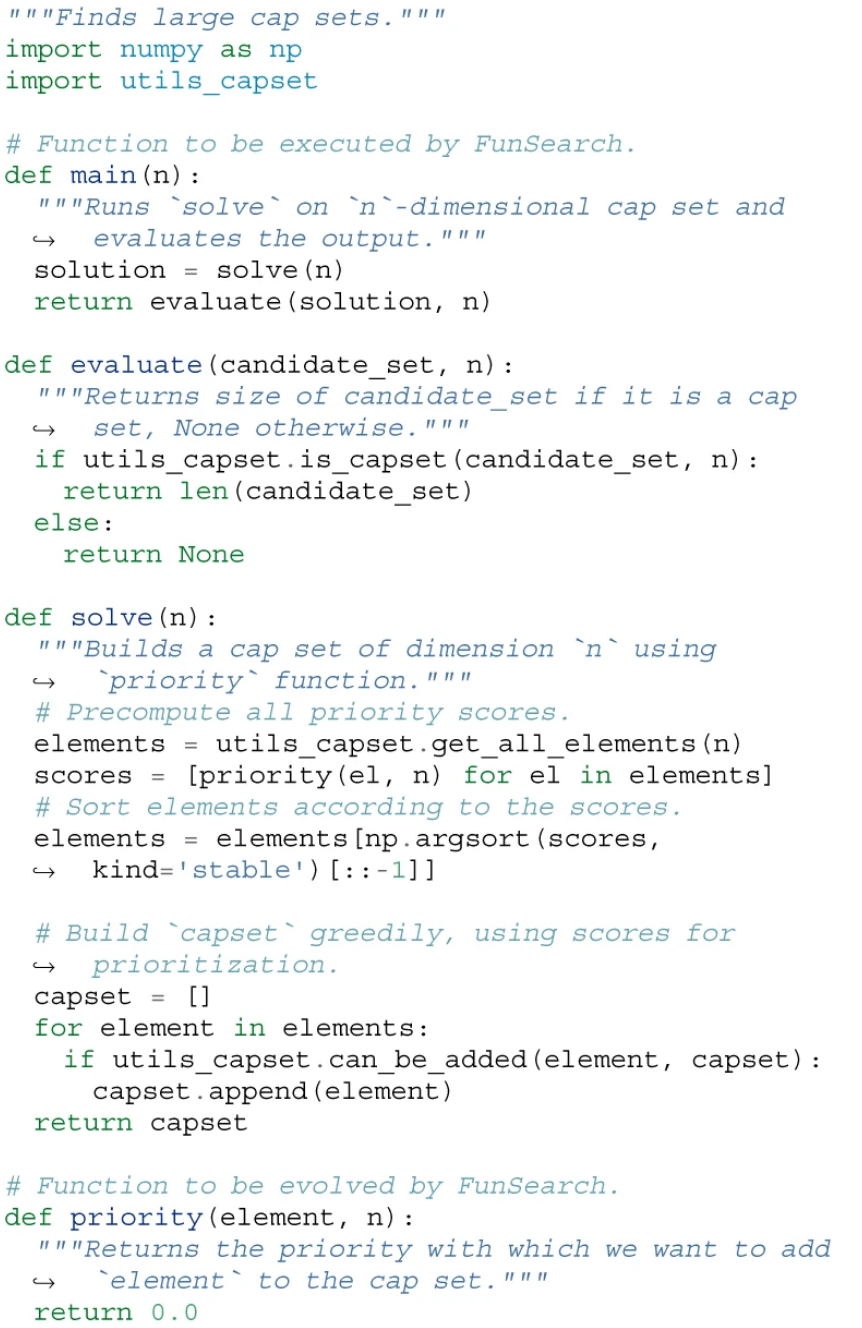
\includegraphics[width=0.5\linewidth]{figures/template.png}
\end{frame}


\begin{frame}{Cap set solution -- the priority function}
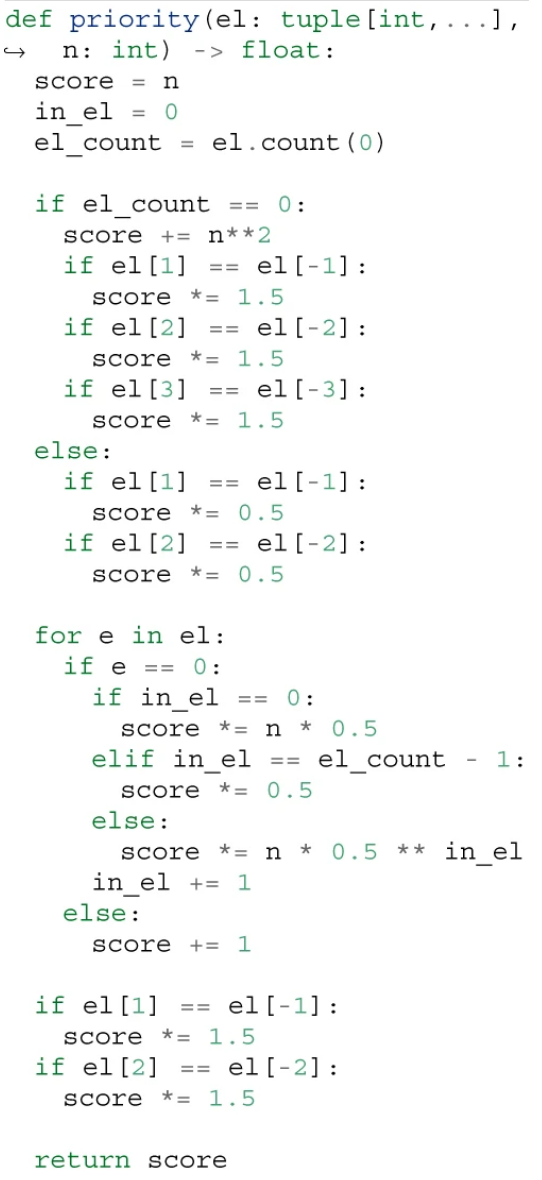
\includegraphics[width=0.3\linewidth]{figures/cup-set-solution.png}
\end{frame}


\begin{frame}{AlphaEvolve}
\textit{tldr}: FunSearch scaled-up in multiple dimensions. \\
\begin{figure}
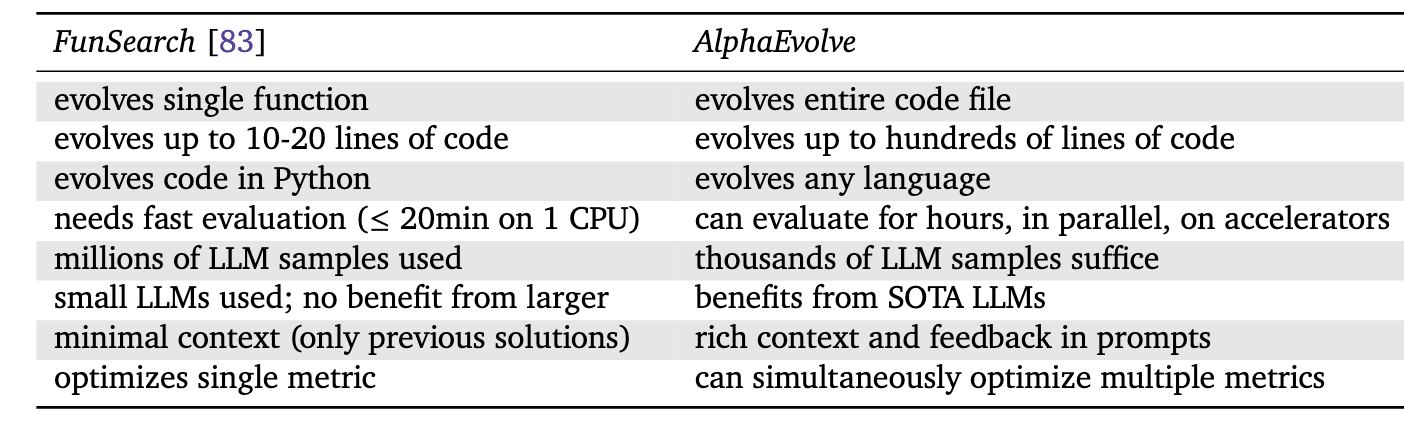
\includegraphics[width=1\linewidth]{figures/funsearch-vs-alphaevolve.png}
\end{figure}
\end{frame}

\begin{frame}{AlphaEvolve -- notable differences}
\begin{itemize}
\item Larger base LLMs (Gemini 2.0 Flash, Gemini 2.0 Pro).
\item Much richer prompts:
\begin{itemize}
\item context for the problem provided,
\item detailed evaluation results included,
\item meta prompt evolution.
\end{itemize}
\item Output format: a \textbf{diff} rather than a new program version.
\item Evaluation:
\begin{itemize}
\item many evaluators,
\item including LLM judges.
\end{itemize}
\item Improved evolution strategy:
\begin{itemize}
\item different islands (as before),
\item MAP elites algorithm.
\end{itemize}
\end{itemize}

\end{frame}

\begin{frame}{Problems tackled}
50 mathematical problems:
\begin{itemize}
\item Fast matrix multiplication, kissing number problem, \ldots
\item For 75\% problems AlphaEvolve matched the optimal known solution.
\item For 20\% problems AlphaEvolve found better solution.
\end{itemize}
Also practical problems related to computational infrastructure:
\begin{itemize}
\item Scheduling jobs on a cluster, optimizing JAX kernel, \ldots
\item Some of the solutions found by AlphaEvolve went into production at Google.
\end{itemize}

\end{frame}

\begin{frame}{Optimizing matrix multiplications}
\begin{itemize}
\item The simple algorithm for multiplying $n \times m$ and $m \times k$
matrices requires $nmk$ scalar multiplications.
\item But Volker Strassen in 1969 showed it can be done with fewer
multiplications.
\item The optimal algorithm in general not known.
\item AlphaEvolve found improvements for multiple specific cases.
\end{itemize}
\begin{figure}
\centering
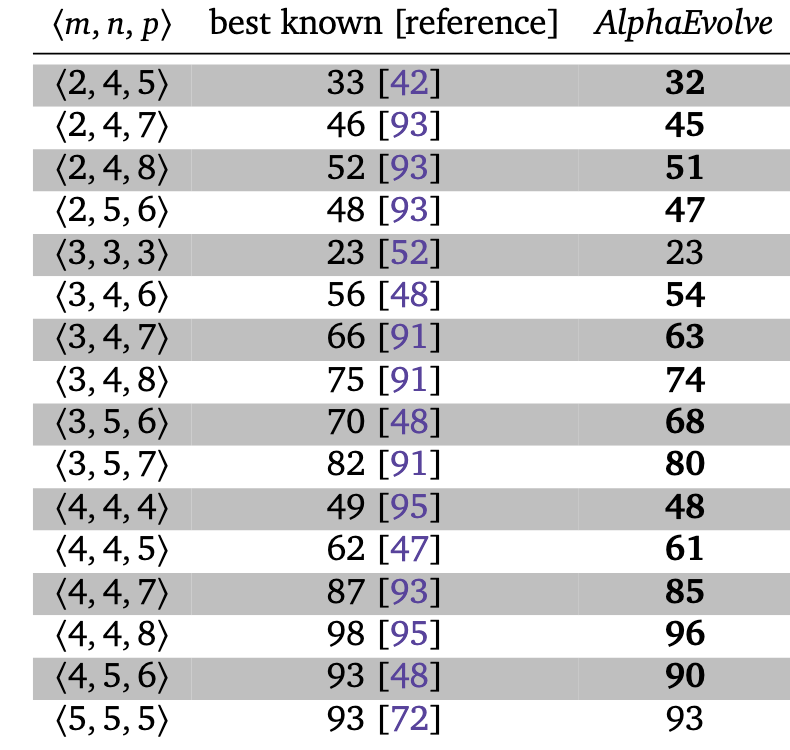
\includegraphics[width=0.5\linewidth]{figures/matmul-table.png}
\end{figure}
\end{frame}

\begin{frame}{Ablations}
\begin{figure}
\centering
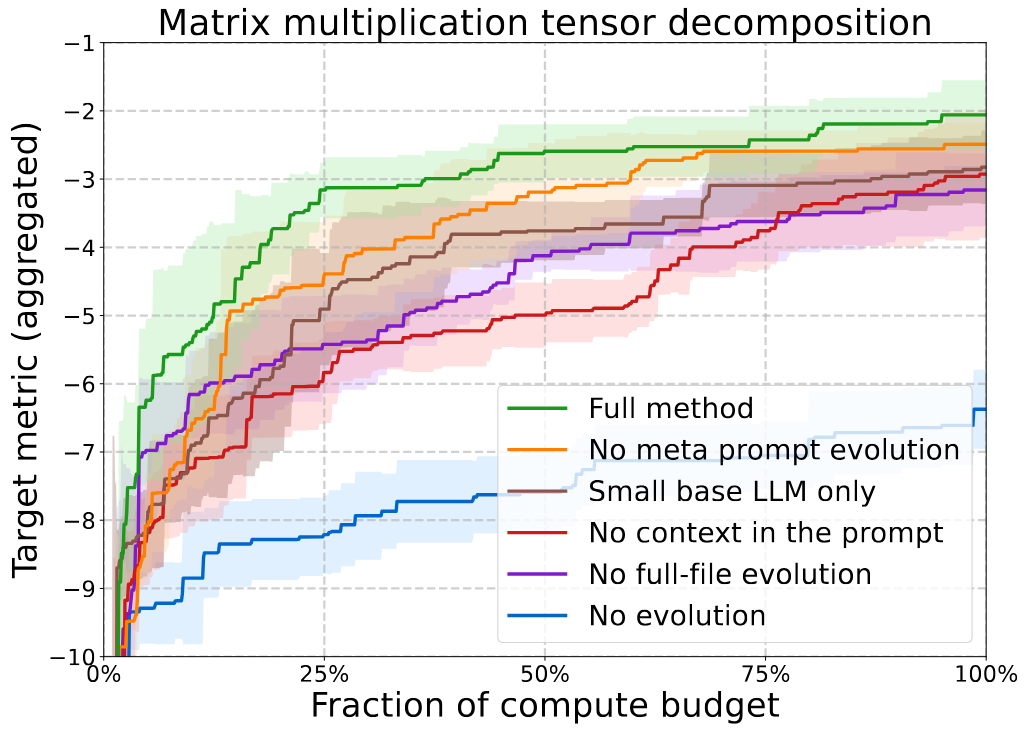
\includegraphics[width=0.8\linewidth]{figures/alphaevolve-ablations.png}
\end{figure}
\end{frame}

\begin{frame}{Closing remarks}
\begin{itemize}
\item FunSearch/AlphaEvolve can be seen as:
\begin{itemize}
\item mechanizing effective interaction with the LLM,
\item complex meta-generation framework.\footnote{See a nice NeurIPS tutorial:\\
\textit{Beyond Decoding: Meta-Generation Algorithms for Large Language Models}}
\end{itemize}
\item An interesting trade-off:
\begin{itemize}
\item smaller, less clever, but faster LLM = more samples (FunSearch) \textit{vs}
\item larger, more clever, but slower LLM = higher-quality samples (AlphaEvolve).
\end{itemize}
\item Can we adapt the AlphaEvolve to formal proving?
    \begin{itemize}
    \item A notion of \textit{partial proof progress} would be needed.
    \item But isn't it similar to what Seed Proved does at test time?
    \end{itemize}
\item Is AlphaEvolve approach better than, say, GRPO fine-tuning?
\item AlphaEvolve could be distilled into a better base LLM, which would result
in \textit{meta-evolution}.
\item Open-source implementation: OpenEvolve.
\end{itemize}
\end{frame}


\end{document}
